\chapter{Overview}


\section{Traditional measuring methods}
Human body can be measured using many different approaches. All of these have their advantages and disadvantages. In this thesis we only need to introduce two of them.

\subsubsection{Hand measurement}
This is the traditional method of using tape measure for obtaining measurements. This approach usually needs one extra person that performs the measurement on the subject. This way the measurements are more precise than the subject using the tape measure without help. The measurements however have to be taken at specific locations to provide correct information in further processing. The locations vary depending on the use and thus there is no universal guide for their measurement. Whereas the professionals are familiar with them, the subjects are usually not as informed. This creates space for human error we are trying to avoid.

\subsubsection{Digital measuring on 3D model}
This method is mentioned because BodyM dataset uses this method to provide ground truth values. Is it based on photogrammetry scanner which creates precise meshes of scanned object. After the human body get acquired from the scanner they are registered to SMPL \cite{smpl} mesh topology. We can then use the resulting mesh for calculating the measurements.


\section{Obstacles}
One of the issues when working with human body measurements is the lack of real world data. The process of measuring is time-consuming and requires privacy measures to take place to protect subjects' personal information. This can be avoided by using synthetic datasets.\\
Moreover the time complexity to train a neural network can be reduced by using powerful device which is not available.


\section{Problem specification}
The goal of this thesis is to expand on body measurements estimation with the use of neural networks. Mainly to explore different data augmentation methods to provide better results when training is done on synthetic dataset.


\section{SMPL}
SMPL is short for Skinned Multi-Person Linear model. This model is based on skinning and blend shapes. The model has been trained on thousands of 3D body scans to create a realistic human model. Full explanation of functions and workflow of this model is out of scope of this work.


\section{Neural network}
Neural network is code built on premises of how human brains work. It consists of connected nodes called neurons. Each neuron takes input variables, processes them and then sends the result to other neurons. Every connection has associated weight which determines the influence said value will have.
Neurons are then organised into layers. They are usually divided into input, output and hidden layers. The function of the hidden layers is to perform the operations needed to calculate output from the input data.
The process of training adjusts the weights of the connections. This automatic process of adjusting is usually based on comparing the output and correct value we provide for the network and minimising the difference.
This process helps the network to find complex relationships or patterns that may not  be as understandable for humans.

\subsubsection{Hyperparameter}
Hyperparameter is a parameter that is not learned but chosen by developer.  These parameters do not change over time. These can be - choice of optimizer, learning rate,  number of layers, filter size and more.\\\\
Our model is mainly built on the following layers:

\subsubsection{Convolution layer}
Most popularly used with convolutional neural networks \cite{convolutional} this layer plays important role in network's functionality. It is based on working with matrices called kernels.  The values in kernel are learnable, which means they are adjusted over the training process to enhance performance. In this thesis we will be using these hyperparameters:
\begin{itemize}
	\item \textbf{Depth} determines dimension of the output volume (activation maps). Influences pattern recognition as well as number of neurons.
	\item \textbf{Size} determines dimensions of kernel.
	\item \textbf{Activation function}
\end{itemize}
The algorithm consists of sliding kernel along the input. At every position it calculates the sum of element-wise multiplication of corresponding pixels in input and kernel. The result is then inserted into the output. This process is then repeated over the whole input multiple times (depending upon number of kernels) %CHECK THIS WHOLE PART PLEASE 
Result of this operation captures local patterns while preserving positional relationships.


\subsubsection{Max Pooling layer}
Max pooling is an operation of non-linear down-sampling. This means that the output image of this layer is usually smaller than the input. This helps to reduce parameters for next convolutional layer, providing faster training.  This layer is defined by two hyperparameters:

\begin{itemize}
	\item \textbf{Filter size} determines the dimensions. In case of the filter reaching out of the array, only valid values are taken into consideration.
	\item \textbf{Stride} determines how many columns will the filter move.
\end{itemize}

The higher these hyperparameters' values are the smaller will the output be.\\
%CHECK IF FIELD IS THE CORRECT TERM
This layer iterates over input field and looks at subfield with size of filter size. In this subfield it finds the largest number and writes only the largest number into the output field. After this, the filter moves by stride columns left until all columns were checked. In that case the filter moves back to first column of the input field and then moves down by the stride (refer to \ref{maxPooling} as an example).\\ This process is repeated until whole input field is iterated.

\begin{figure}
	\centering{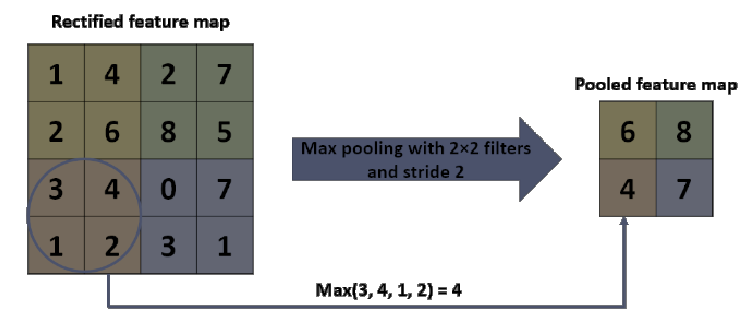
\includegraphics[scale=0.4]{images/MaxPoolingExample}}
	\caption[Max Pooling Example]{Max Pooling Example \cite{pooling}}
	\label{maxPooling}
\end{figure}

\subsubsection{Overfitting}
\section{Keras \cite{keras}}
Keras is an open-source neural network library written in Python. Thanks to its user-friendly interface and modular design is Keras one of the leading frameworks in neural network development. Its simple yet flexible architecture allows for easy prototyping and experimentation, making it an ideal choice for both beginners and experienced practitioners in the field of deep learning.
\section{OpenCV \cite{opencv}}
Open Source Computer Vision Library (OpenCV for short) is a comprehensive open-source library originally developed by Intel. It is mainly used for various tasks in fields such as computer vision or machine learning. In the time of writing this thesis, OpenCV provides over 2500 optimized algorithms. These are able to effectively perform many tasks such as face detection, object tracking, image preprocessing and many more. Providing interfaces in multiple programming languages such as Python, C++, Java and MATLAB it is very popular with community as well as recognisable and famous companies.%Add reference?

\section{Photogrammetry}

%\begin{figure}
%	%vlozenie samotneho obrazku vycentrovaneho a vhodnej velkosti
%	%obrazok je v subore images/cervik.png
%	\centering{\includesvg[scale=0.7]{images/DatasetComparation}}
%	%popis obrazku
%	\caption[Ukážka hry Červík]{Ukážka hry Červík. Červík je znázornený červenou farbou, voľné políčka sivou, jedlo zelenou a steny čiernou. Hoci tento popis obrázku je dlhší, v zdrojovom texte je aj kratšia verzia, ktorá sa zobrazí v zozname obrázkov.}
%	%id obrazku, pomocou ktoreho sa budeme na obrazok odvolavat
%	\label{fig:beep}
%\end{figure}\includegraphics